% !TEX root = ../main.tex
\chapter{Introduction}
\label{chapter:Introduction}
	This document has been created in order to show you some of the capabilities 
of \LaTeX.  A great resource for an introduction to \LaTeX\xspace is Tobias
Oetiker's ''The Not So Short Introduction to \LaTeXe'' \cite{latex}.  Please
page through that document
before starting with your thesis.
Oh, and let's use the mysterious word \gls{computer} here to give the glossary
a reason to appear.
A third useful option to reference stuff besides citing or glossarying (?) 
is using footnotes. Just like
this\footnote{Properly formatted clickable URL: \url{https://www.tum.de/}}
one.
And: lists! Lists with bullet points are amazing. I mean, just look at this:
\begin{itemize}
	\item list
	\item all 
	\item the 
	\item things!
\end{itemize}
% use enumerate for numbers instead of points: 
% https://en.wikibooks.org/wiki/LaTeX/List_Structures#List_structures
\par
Anyways your introduction goes here.


Below a few \LaTeX examples are included for beginners
\comment{You can also put comments in the margins for you or your advisor}
\begin{figure}[ht]
  \centering
  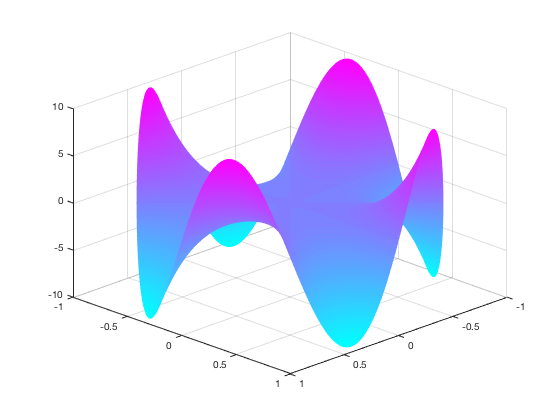
\includegraphics[width=5cm]{images/swing_function_plot.png}
  \caption{$u(x)$}%{Numerically solved solution}
  \label{fig:swingPlot}
\end{figure}


Equations can also be labeled
\begin{equation}
	\pi = \mathrm{e}^{i\cdot\phi}
	\label{eq:equation1}
\end{equation}


And later referenced. Even in subfigures.
\begin{figure}[!htb]
  \centering
  \begin{subfigure}[b]{0.3\textwidth}
    \centering
  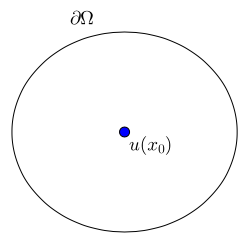
\includegraphics[width=\textwidth]{images/CircCenter}
  \caption{Equation \ref{eq:equation1}}\label{fig:circcenter}
\end{subfigure}
\hfill
  \begin{subfigure}[b]{0.3\textwidth}
    \centering
  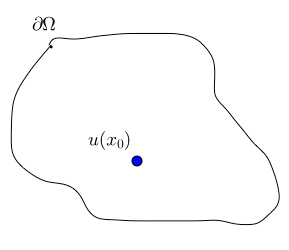
\includegraphics[width=\textwidth]{images/GeneralOffset}
  \label{fig:generaloffset}
  \caption{Equation \ref{eq:equation1}}
\end{subfigure}
\end{figure}
\section{Including code}

Code can be using the package
\href{https://www.sharelatex.com/learn/Code\_Highlighting\_with\_minted}{Minted}.

An exaple of which of can be found below (see Source Code \ref{lst:nice_listing})
\begin{listing}
	%the language syntax can be declared here.
	\begin{minted}{python} 
	import numpy as np
	
	def incmatrix(genl1,genl2):
	    m = len(genl1)
	    n = len(genl2)
	    M = None #to become the incidence matrix
	    VT = np.zeros((n*m,1), int)  #dummy variable
	
	    #compute the bitwise xor matrix
	    M1 = bitxormatrix(genl1)
	    M2 = np.triu(bitxormatrix(genl2),1)
	
	    for i in range(m-1):
	        for j in range(i+1, m):
	            [r,c] = np.where(M2 == M1[i,j])
	            for k in range(len(r)):
	                VT[(i)*n + r[k]] = 1;
	                VT[(i)*n + c[k]] = 1;
	                VT[(j)*n + r[k]] = 1;
	                VT[(j)*n + c[k]] = 1;
	
	                if M is None:
	                    M = np.copy(VT)
	                else:
	                    M = np.concatenate((M, VT), 1)
	
	                VT = np.zeros((n*m,1), int)
	
	    return M
	\end{minted}

  \caption{My nice listing}
  \label{lst:nice_listing}
\end{listing}
